\section{Introduction to binary tree}
\begin{itemize}
    \item In a binary search tree, the elements have a hierarchical relationship or \emph{parent-child} relationship. These are not linear data structures, linked lists, arrays, stacks, queues are all linear because they do not have a hierarchy. 
    \item Any tree has hierarchical relationships. 
\end{itemize}

\subsection{Examples of binary trees}
\begin{itemize}
    \item A tree can have 0,1 or at most two children.
    \item Each child has 0 or 1 parent. 
    \item The root node is the only node that can have no parents. 
    \item A root can have an empty right tree and an empty left tree. 
    \item The definition of binary trees is recursive, since for instance we can remove node $A$ and be left with two trees by themselves, in this case $B$ would be the root for the left tree, and $C$ would be the root for the right tree. 
        \begin{figure}[H]
            \centering
            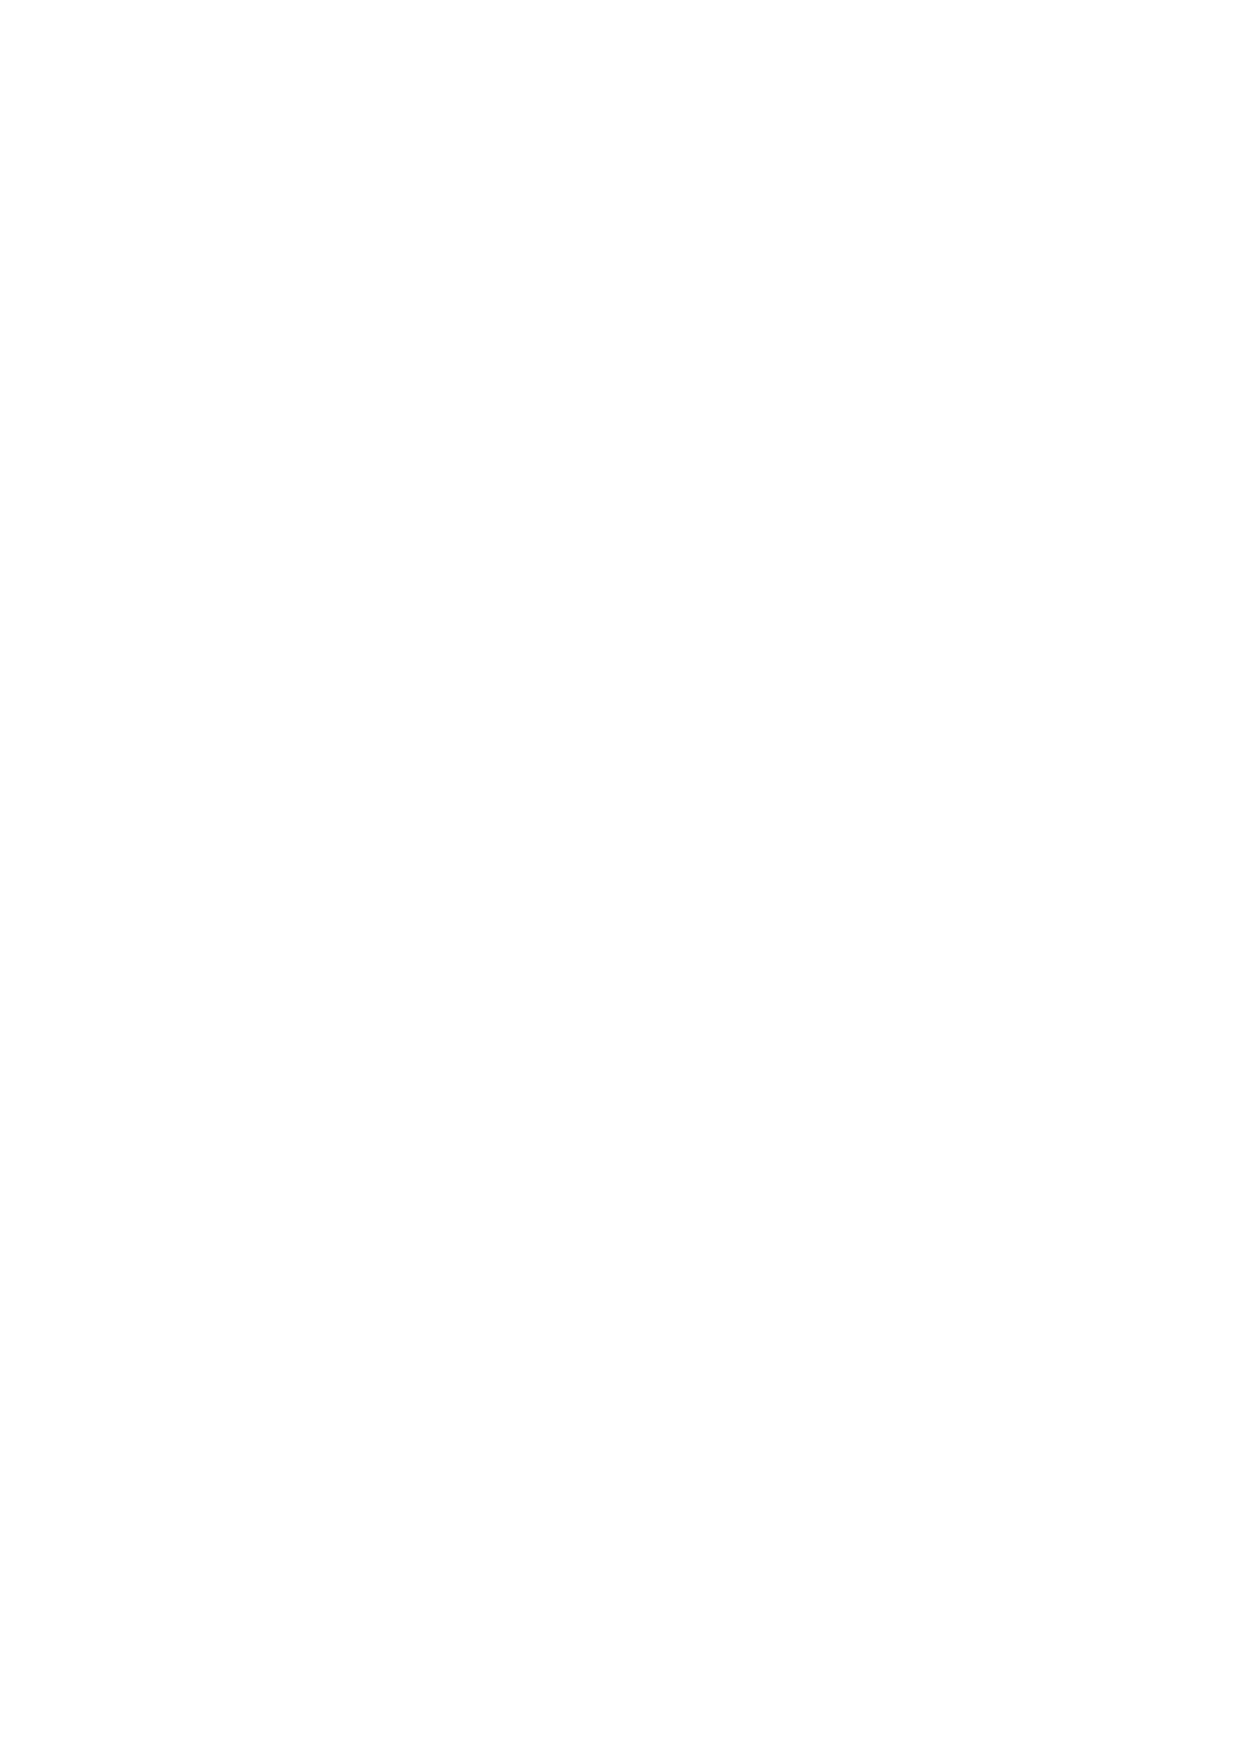
\includegraphics[width=\textwidth]{\figs/binarysearchtreeexample} 
        \end{figure}
\end{itemize}

\subsection{Valid examples and non-valid examples}
\begin{figure}[H]
    \centering
    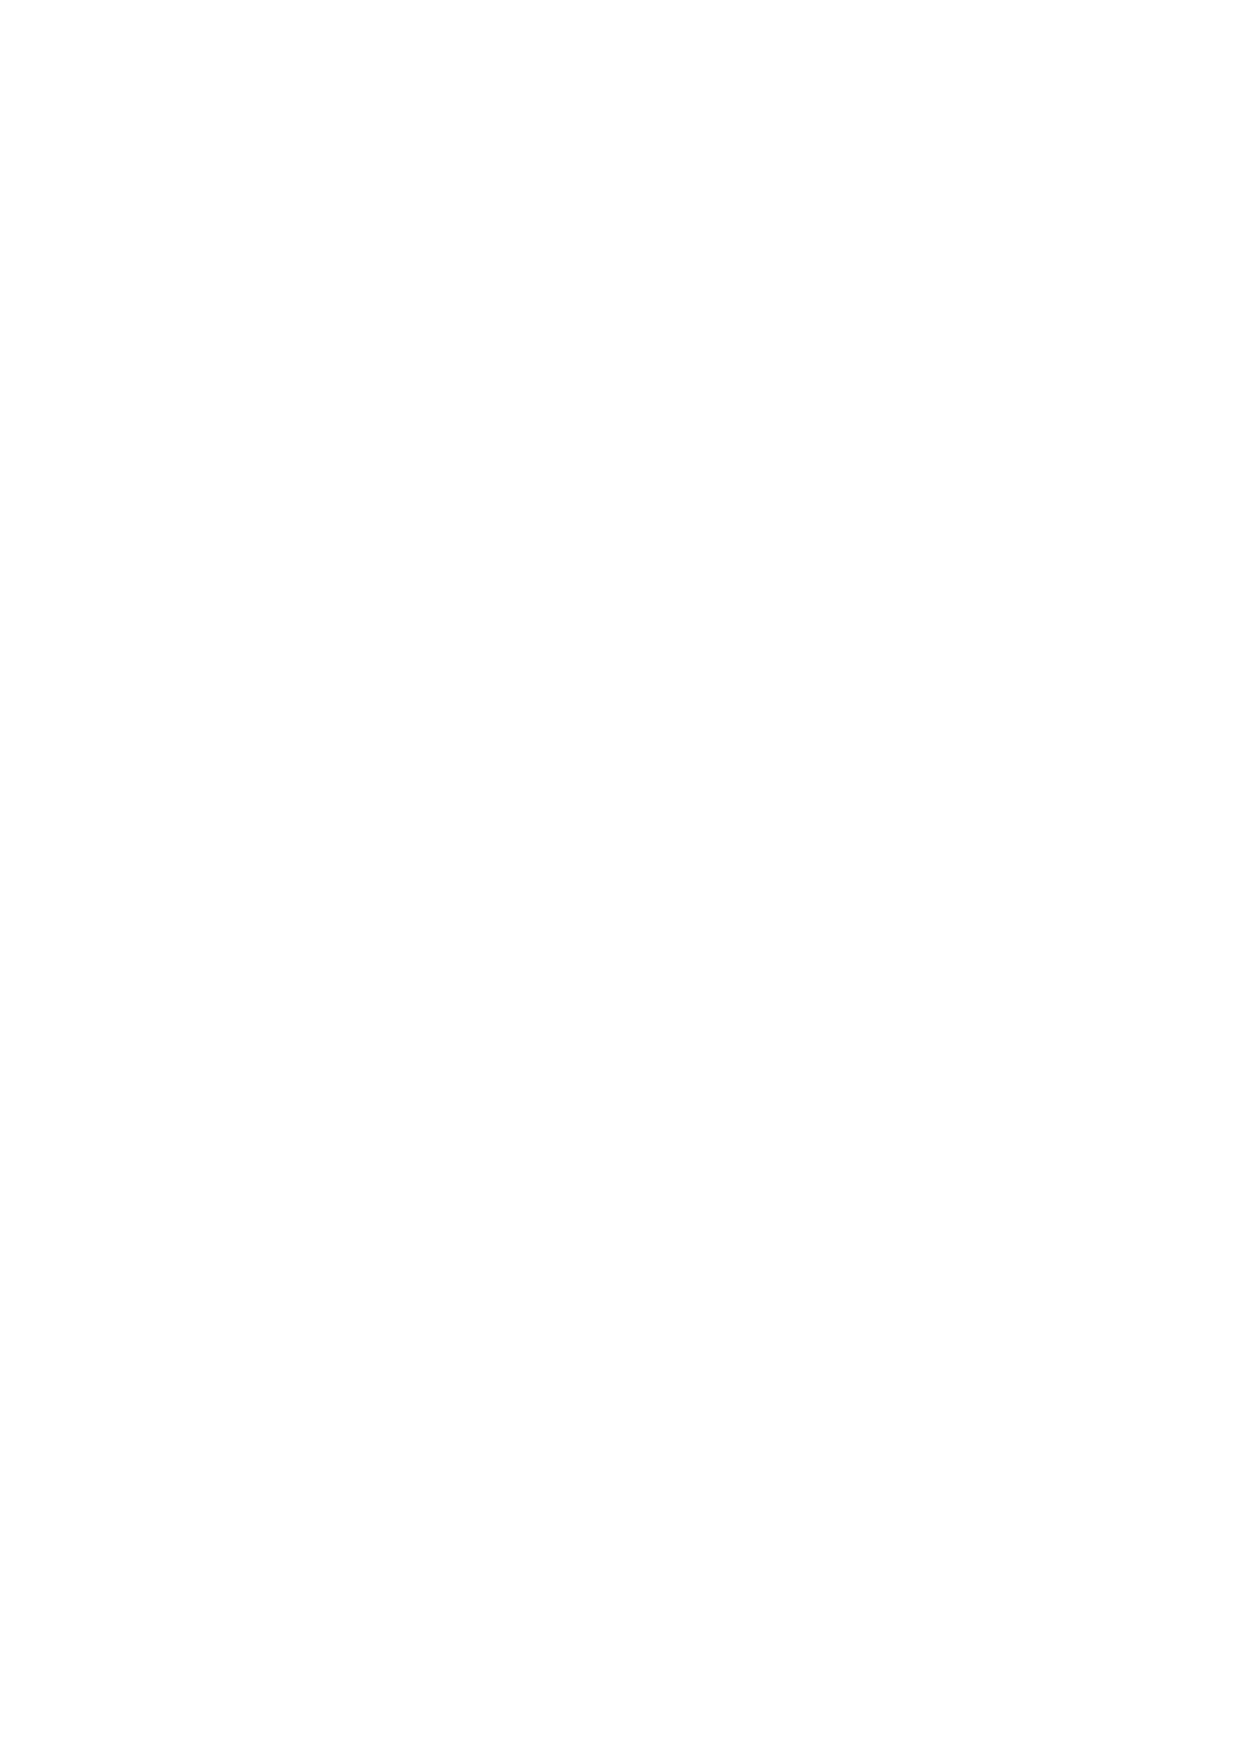
\includegraphics[width=\textwidth]{\figs/binarysearchtree}
\end{figure}

\section{Formal definition}
\termdefinition{Binary tree}{ Binary tree is a set of 3 \emph{disjoint} subsets, the first one is the root of the tree and the other 2 subsets are either empty or they are themselves binary trees.\cite[From Data Structures Using C and C++]{DEusingCCpp}}  


%----------------------------------------------------------------------------------------
\section{Understanding different terminologies related with binary trees}
\begin{itemize}
    \item The root is located at level 0.
    \item The children of any parent node will have a level equivalent to the level of the parent plus one. 
    \item A leaf node or external node is a node that does not have any children.
    \item An internal node is a parent node with two children. 
    \item A half-leaf node is a parent node with only one child.
    \item The height of the binary tree is the level of the leaf that is at the bottom, some books have it as the level of the leafs at the bottom + one. 
    \item Two nodes are considered siblings when they are children of the same parents. 
\end{itemize}

\subsection{Example}
\begin{itemize}
    \item Root is $A$. 
    \item $C,D,F\;\&\;G$ are leaf nodes or external nodes. 
    \item $A,B\;\&\;E$ are internal nodes. 
    \item There are no half-leafs except for node $A$.
    \item The height is 3 (considering start at 0).
    \item $(B,C),(D,E)\;\&\;(F,G)$ are siblings because they have the same parent.
\end{itemize}
\begin{figure}[H]
    \centering
    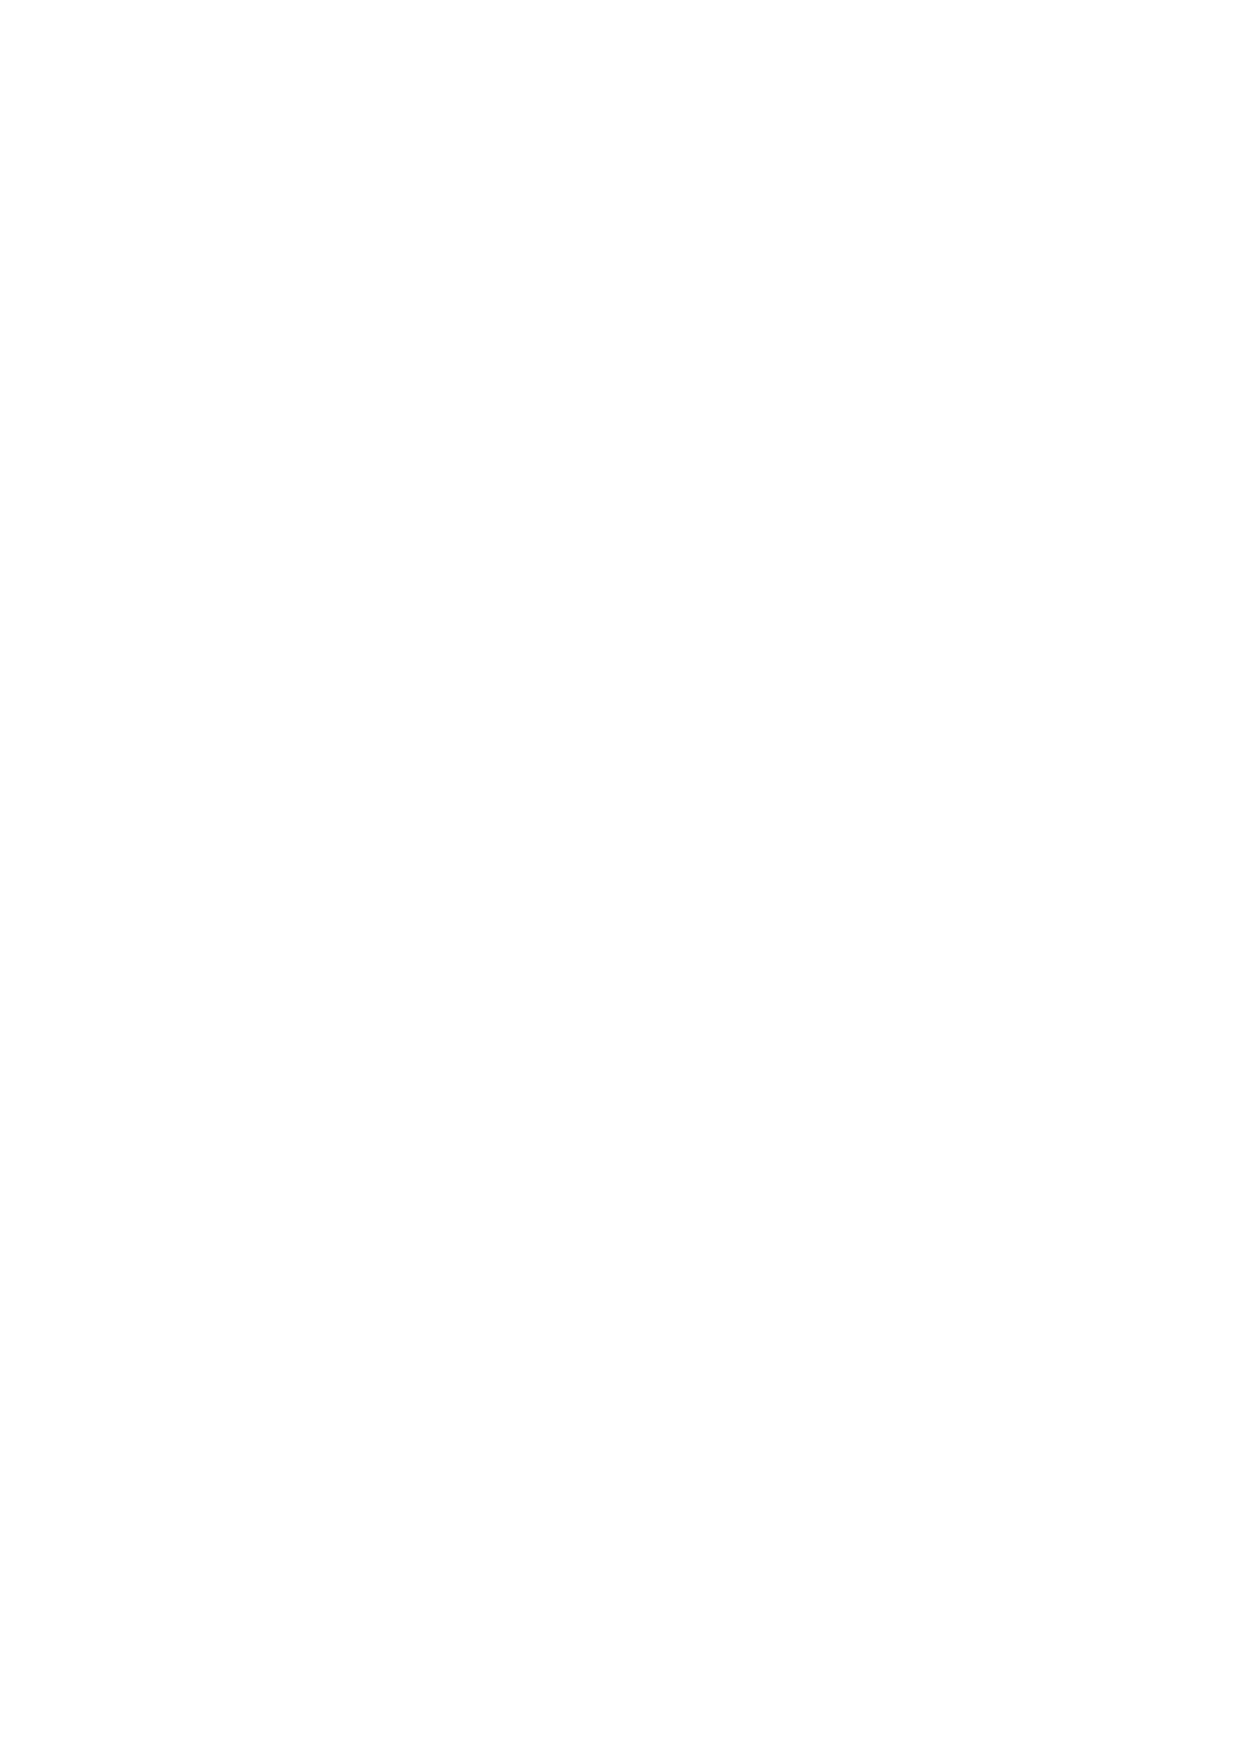
\includegraphics[width=\textwidth]{\figs/binarysearchtreeterminology}
\end{figure}

\section{Two tree / strictly binary tree}
\begin{itemize}
    \item \termdefinition{Two tree or strictly binary tree}{ is a binary tree where each node is either a leaf, or they are having both children. Meaning no half-leaf nodes.} 
\end{itemize}
\begin{figure}[H]
    \centering
    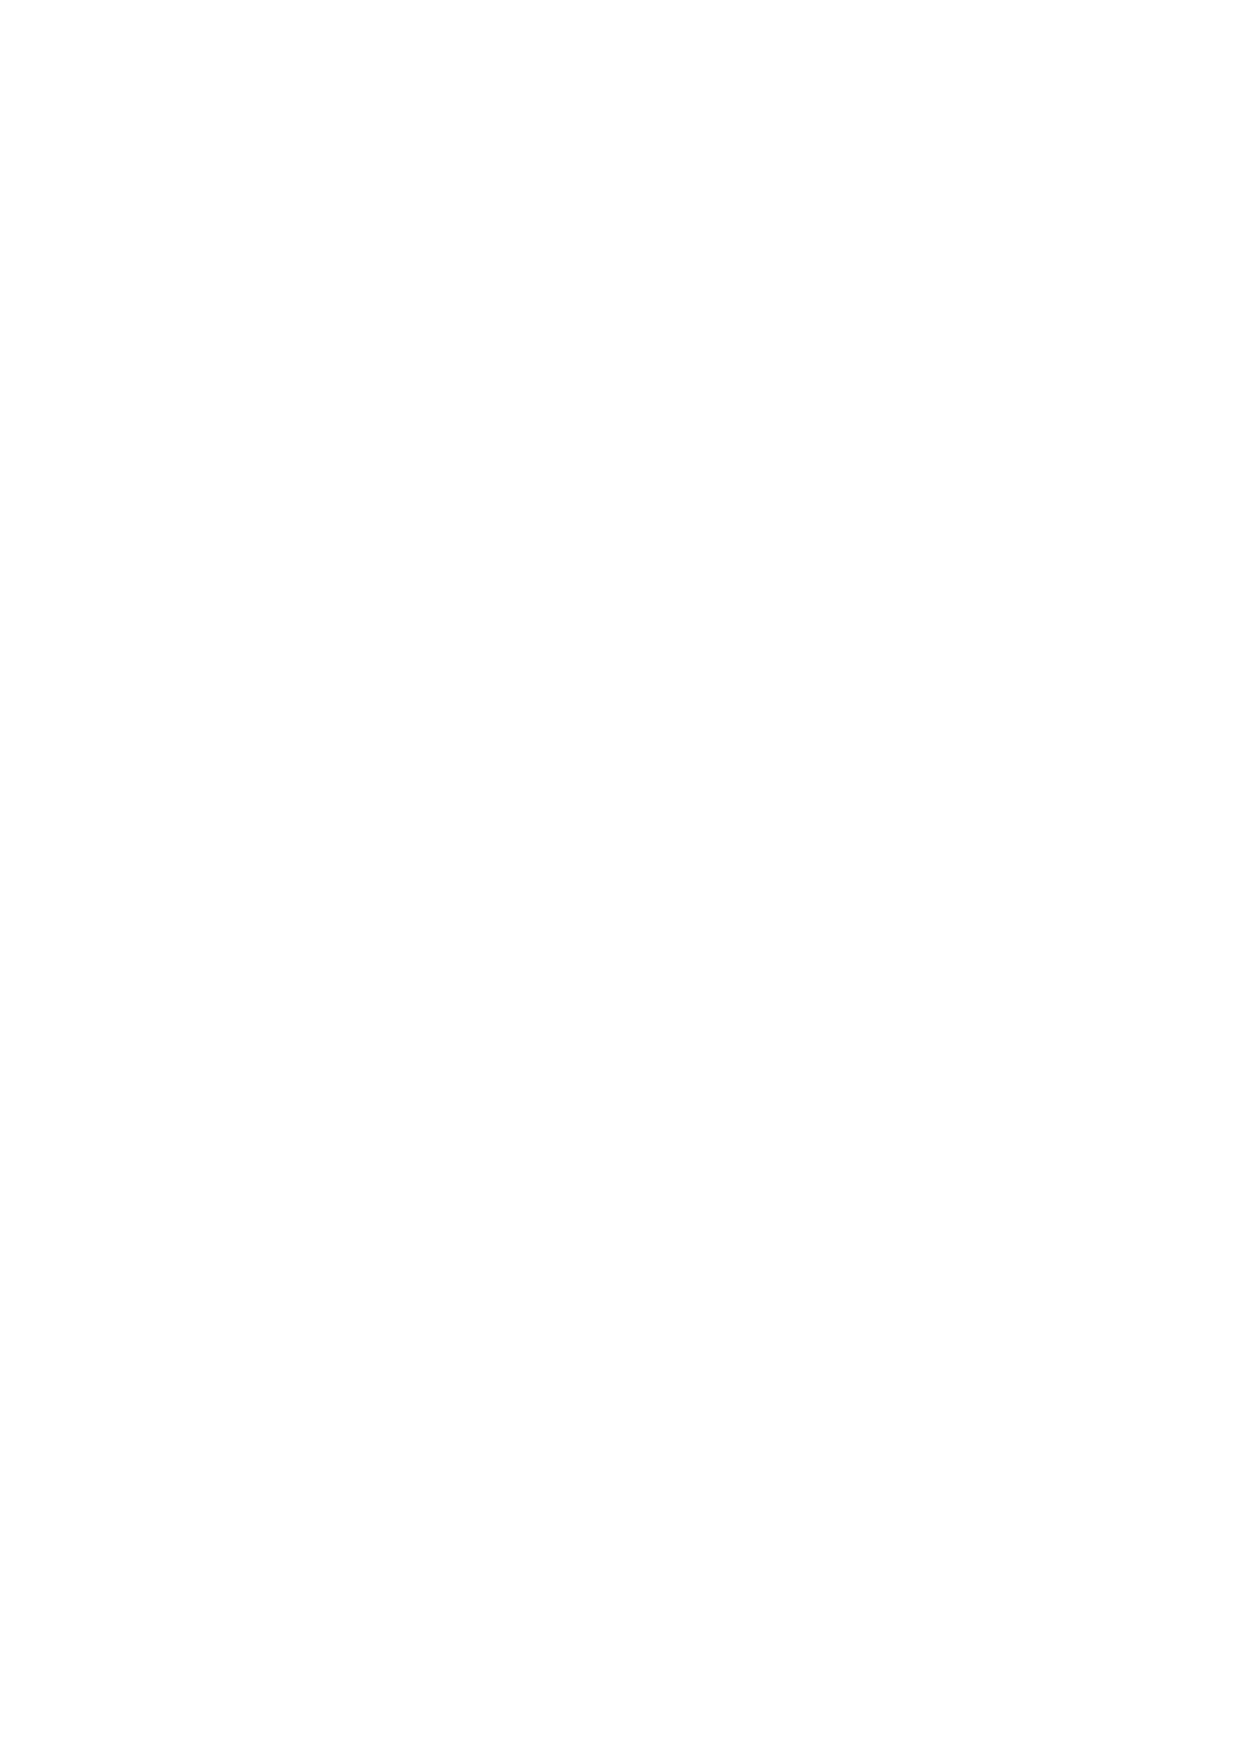
\includegraphics[width=\textwidth]{\figs/strictlybt}
\end{figure}

\section{Complete binary tree / full tree}
\begin{itemize}
    \item \termdefinition{Complete binary tree / full tree }{ A complete binary tree is a 2-tree where all leaves must reside at the same level. OR, in a complete binary tree at any leaf $k$, there are always $2k$ nodes.}
\end{itemize}
\begin{figure}[H]
    \centering
    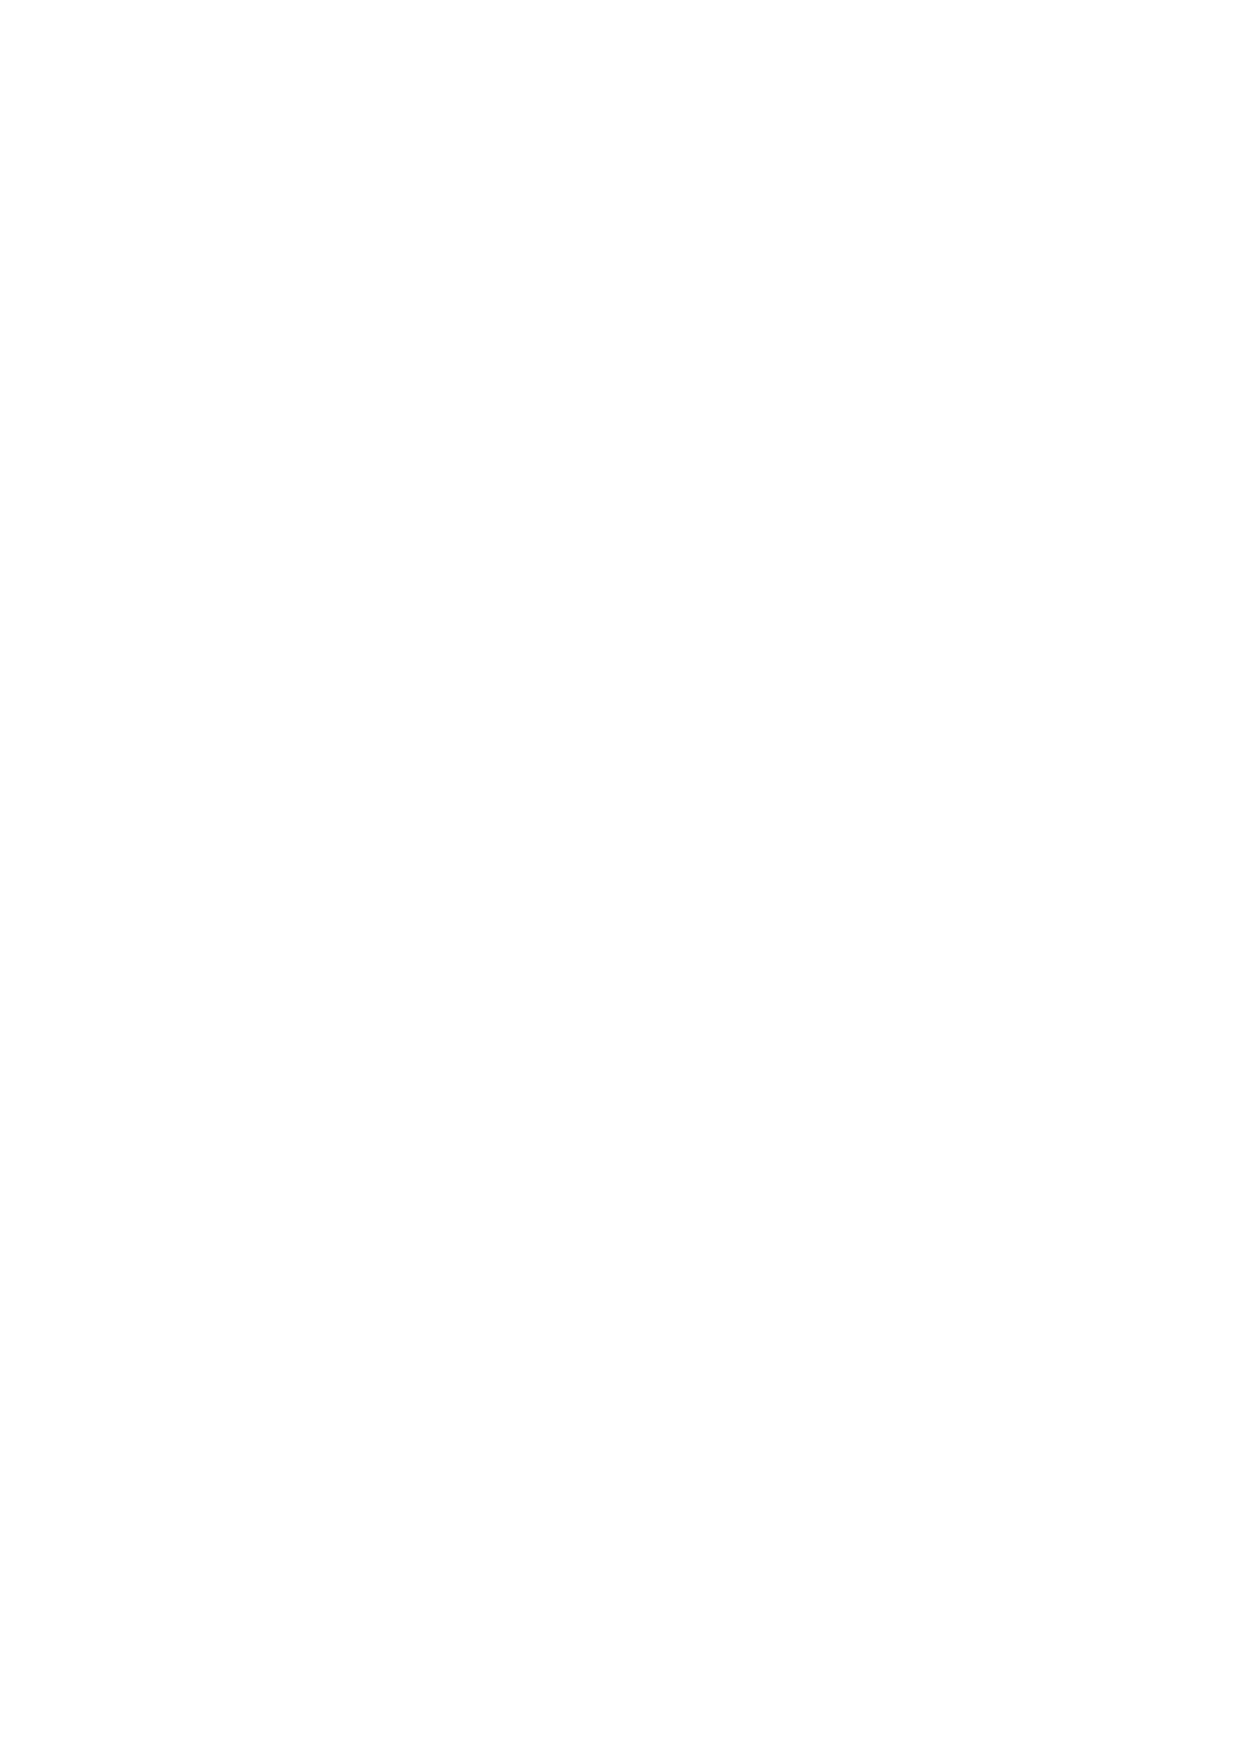
\includegraphics[width=\textwidth]{\figs/completebt}
\end{figure}
\begin{itemize}
    \item The total nodes in a complete binary tree is calculated by: 
        \[
          t_n = 2^{h+1}-1
        \]
        or \[
          t_n = 2^0+2^1+2^2+2^3+\dots+2^h
        \]
        Where the $h$ is the height.
        \begin{itemize}
            \item In the example above is $2^{2+1}-1 = 8-1 = 7$.
        \end{itemize}
    \item To calculate the number of non-leaves.
        \[
          \text{ non-leaves } = 2^h-1
        \]
    
    \item Total leaves: 
        \[
          \text{ total-leaves }=2^h
        \]
\end{itemize}


%----------------------------------------------------------------------------------------
\section{How to traverse a binary tree}
There are three strategies for traversing a binary tree:
\begin{enumerate}
    \item In-order traversal.
    \item Pre-order traversal.
    \item Post-order traversal.
\end{enumerate}
In a binary trees it's impossible to traverse linearly, they are not like arrays or linked lists in the sense where you can do a loop and traverse. Trees are not linear data structures and in order to visit every node of the tree at least once we need to have proper traversal strategies. Whenever we traverse a binary tree we must do it recursively. 

\subsection{In-order traversal strategy}
This strategy consists of implementing a recursive algorithm. This algorithm considers every current node as a sub-tree in itself.
\begin{enumerate}
    \item Traverse the left sub-tree using in-order routine. 
    \item Access root.
    \item Traverse right sub-tree using in order routine.
\end{enumerate}
\begin{figure}[H]
    \centering
    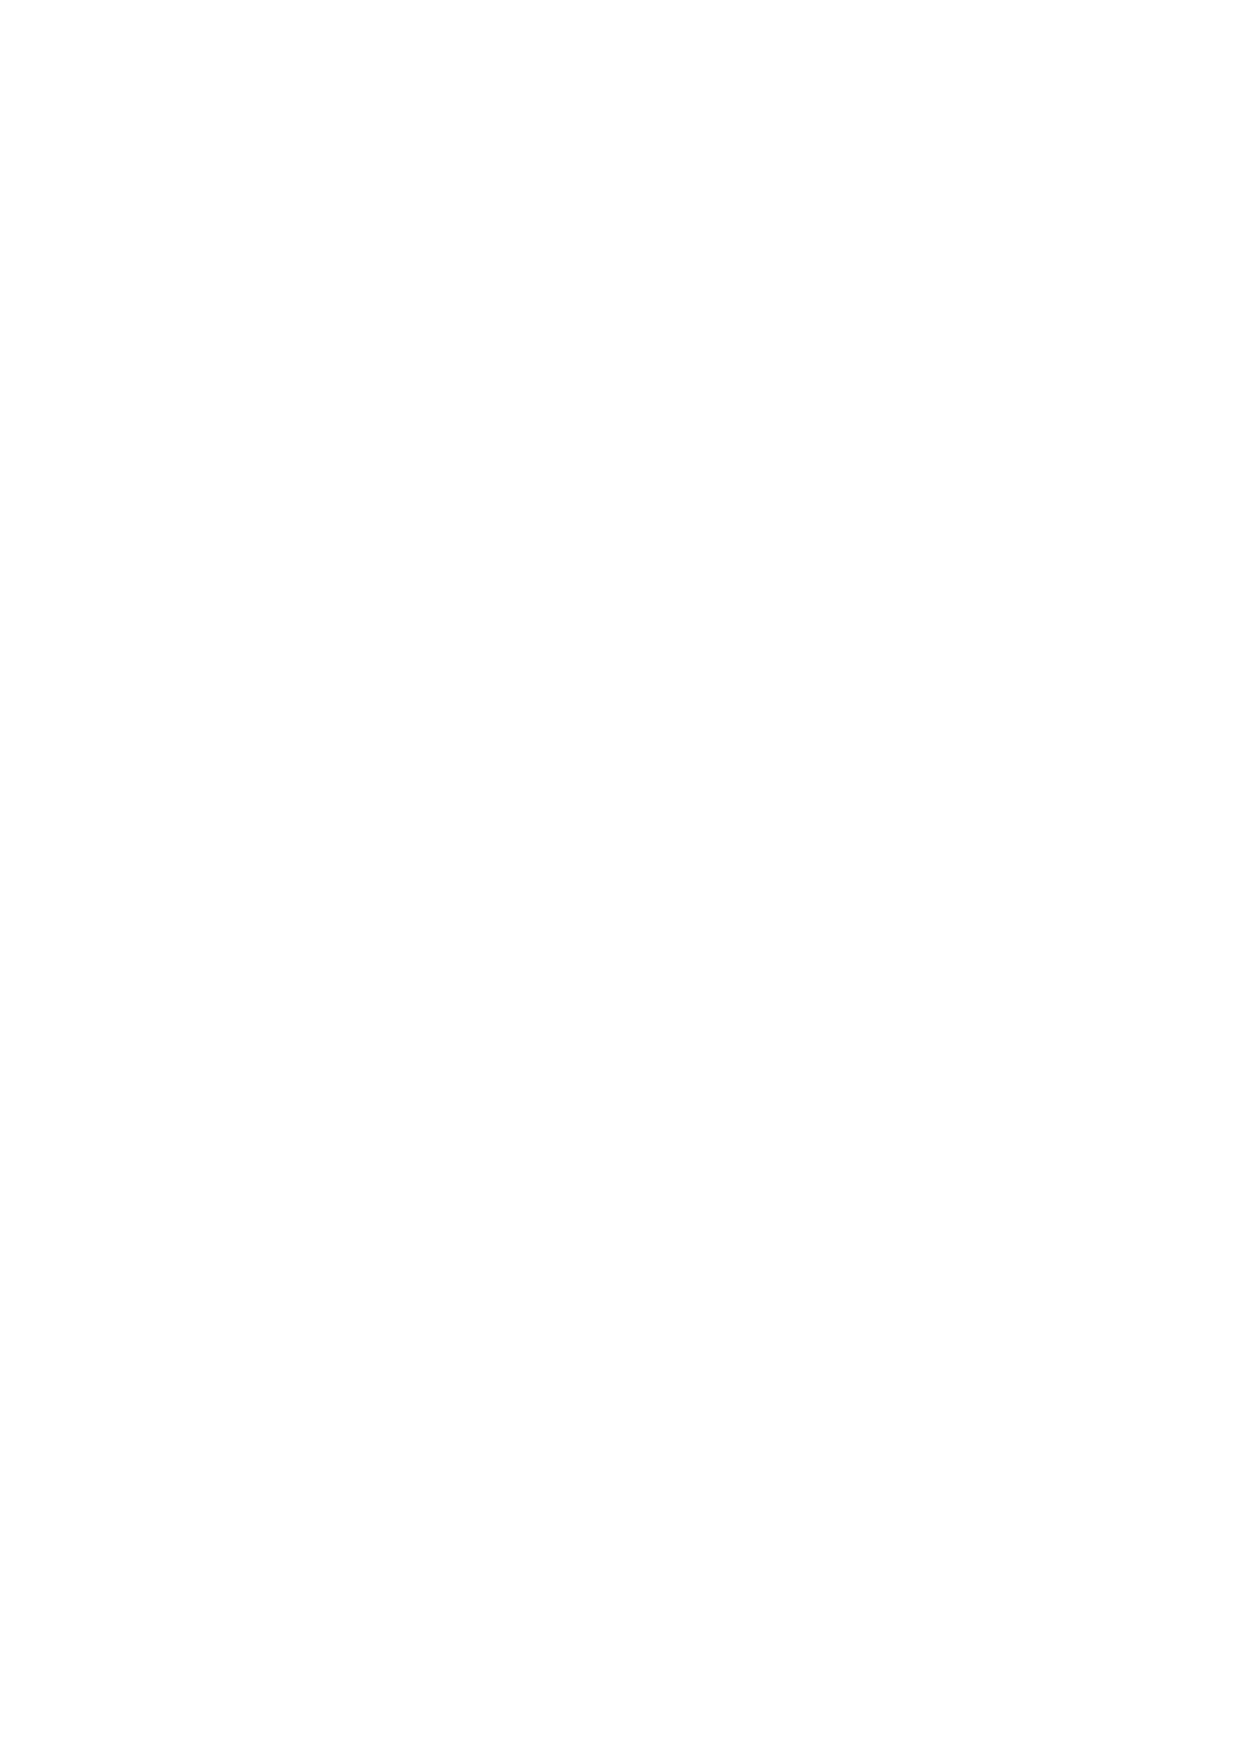
\includegraphics[scale=1.1]{\figs/inordertraversal}
\end{figure}


%----------------------------------------------------------------------------------------
\subsection{Pre-order traversal strategy}
It's different from the in-order because here the root stays constant, this algorithm doesn't consider each node the root.
\begin{enumerate}
    \item Access the root. 
    \item Traverse left sub-tree using the pre-order algorithm using recursion. 
    \item Traverse right-sub-tree using pre-order.
\end{enumerate}
\begin{figure}[H]
    \centering
    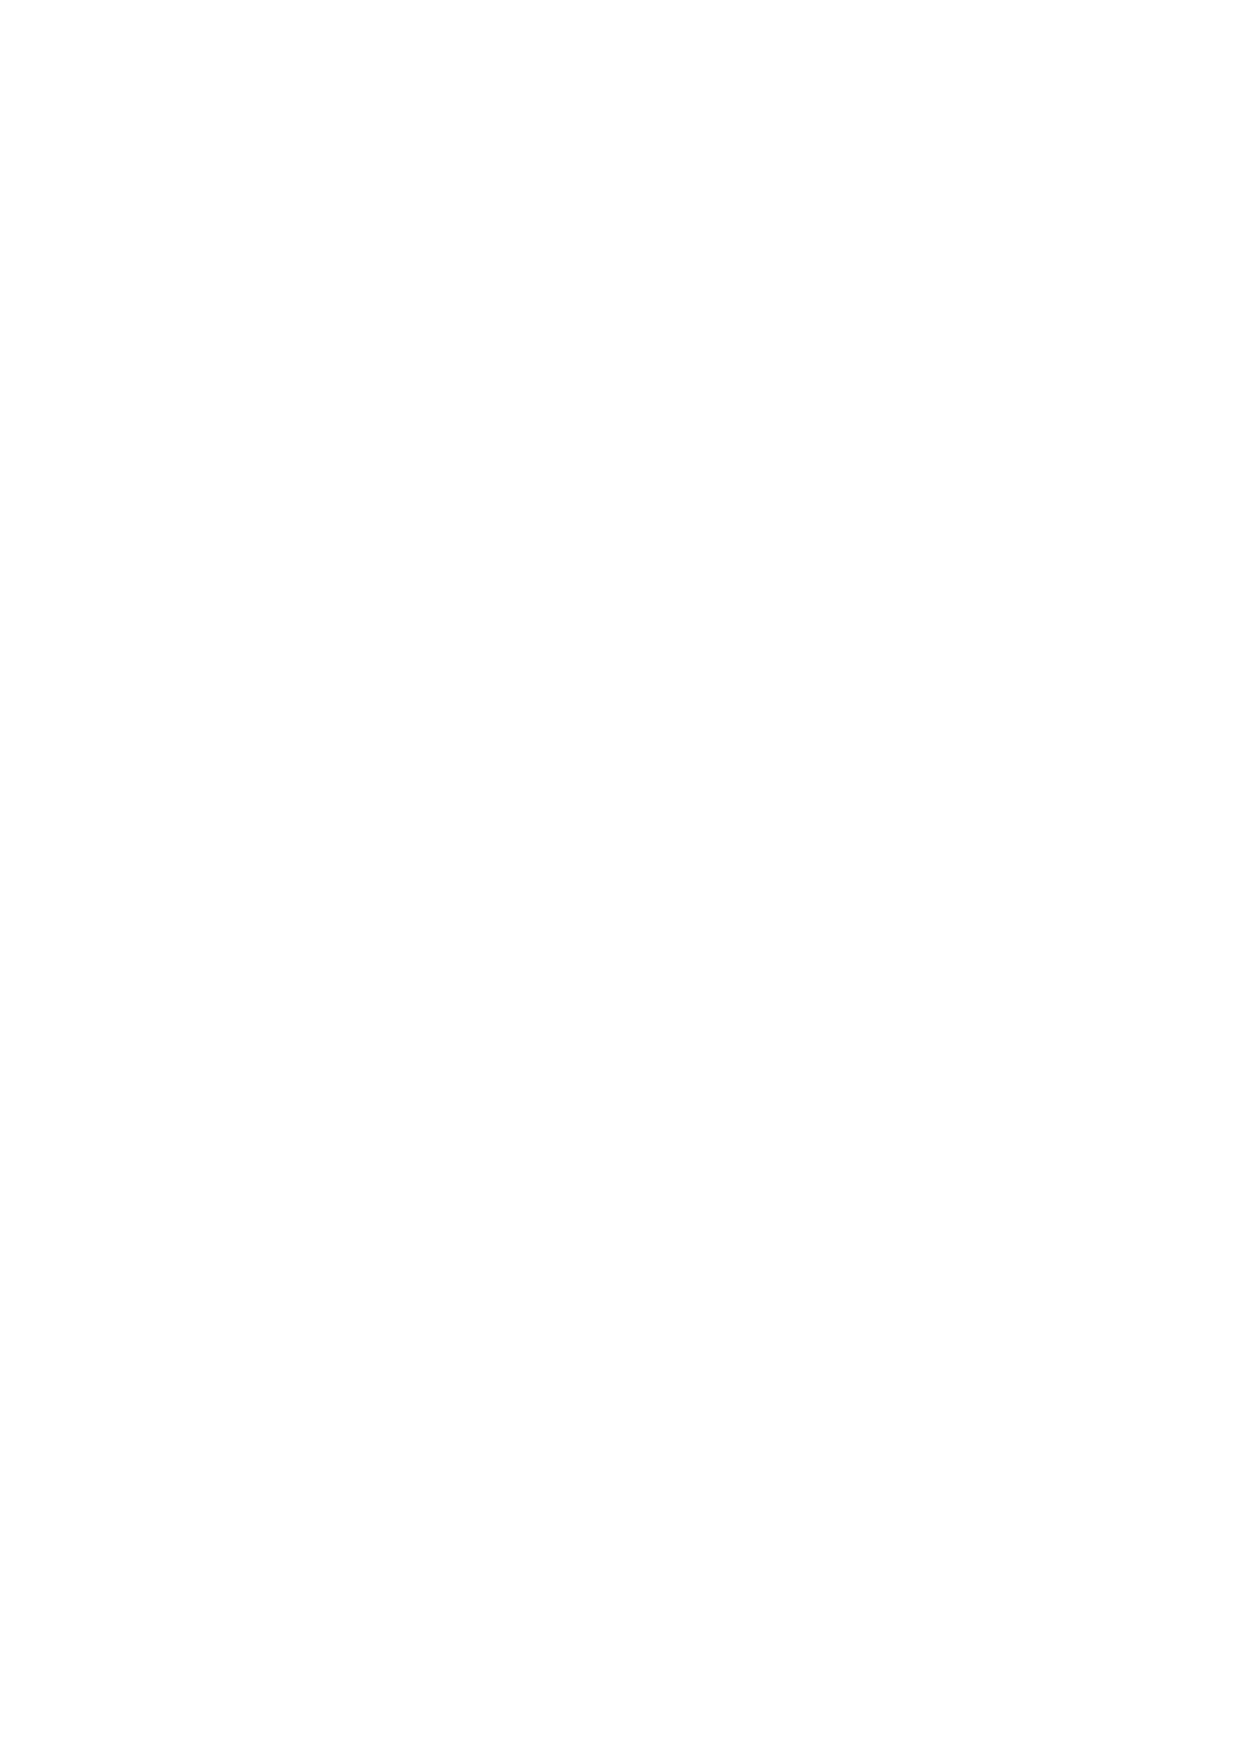
\includegraphics[scale=1.1]{\figs/preorderbt}
\end{figure}


%----------------------------------------------------------------------------------------
\subsection{Post-order traversal strategy}
In this implementation the root is accessed at the end. The position where we access the root is at the end. This is also recursive. 
\begin{enumerate}
    \item Traverse the left-sub-tree using post-order. 
    \item Traverse the right-sub-tree using post-order.
    \item Access the root.
\end{enumerate}
\begin{figure}[H]
    \centering
    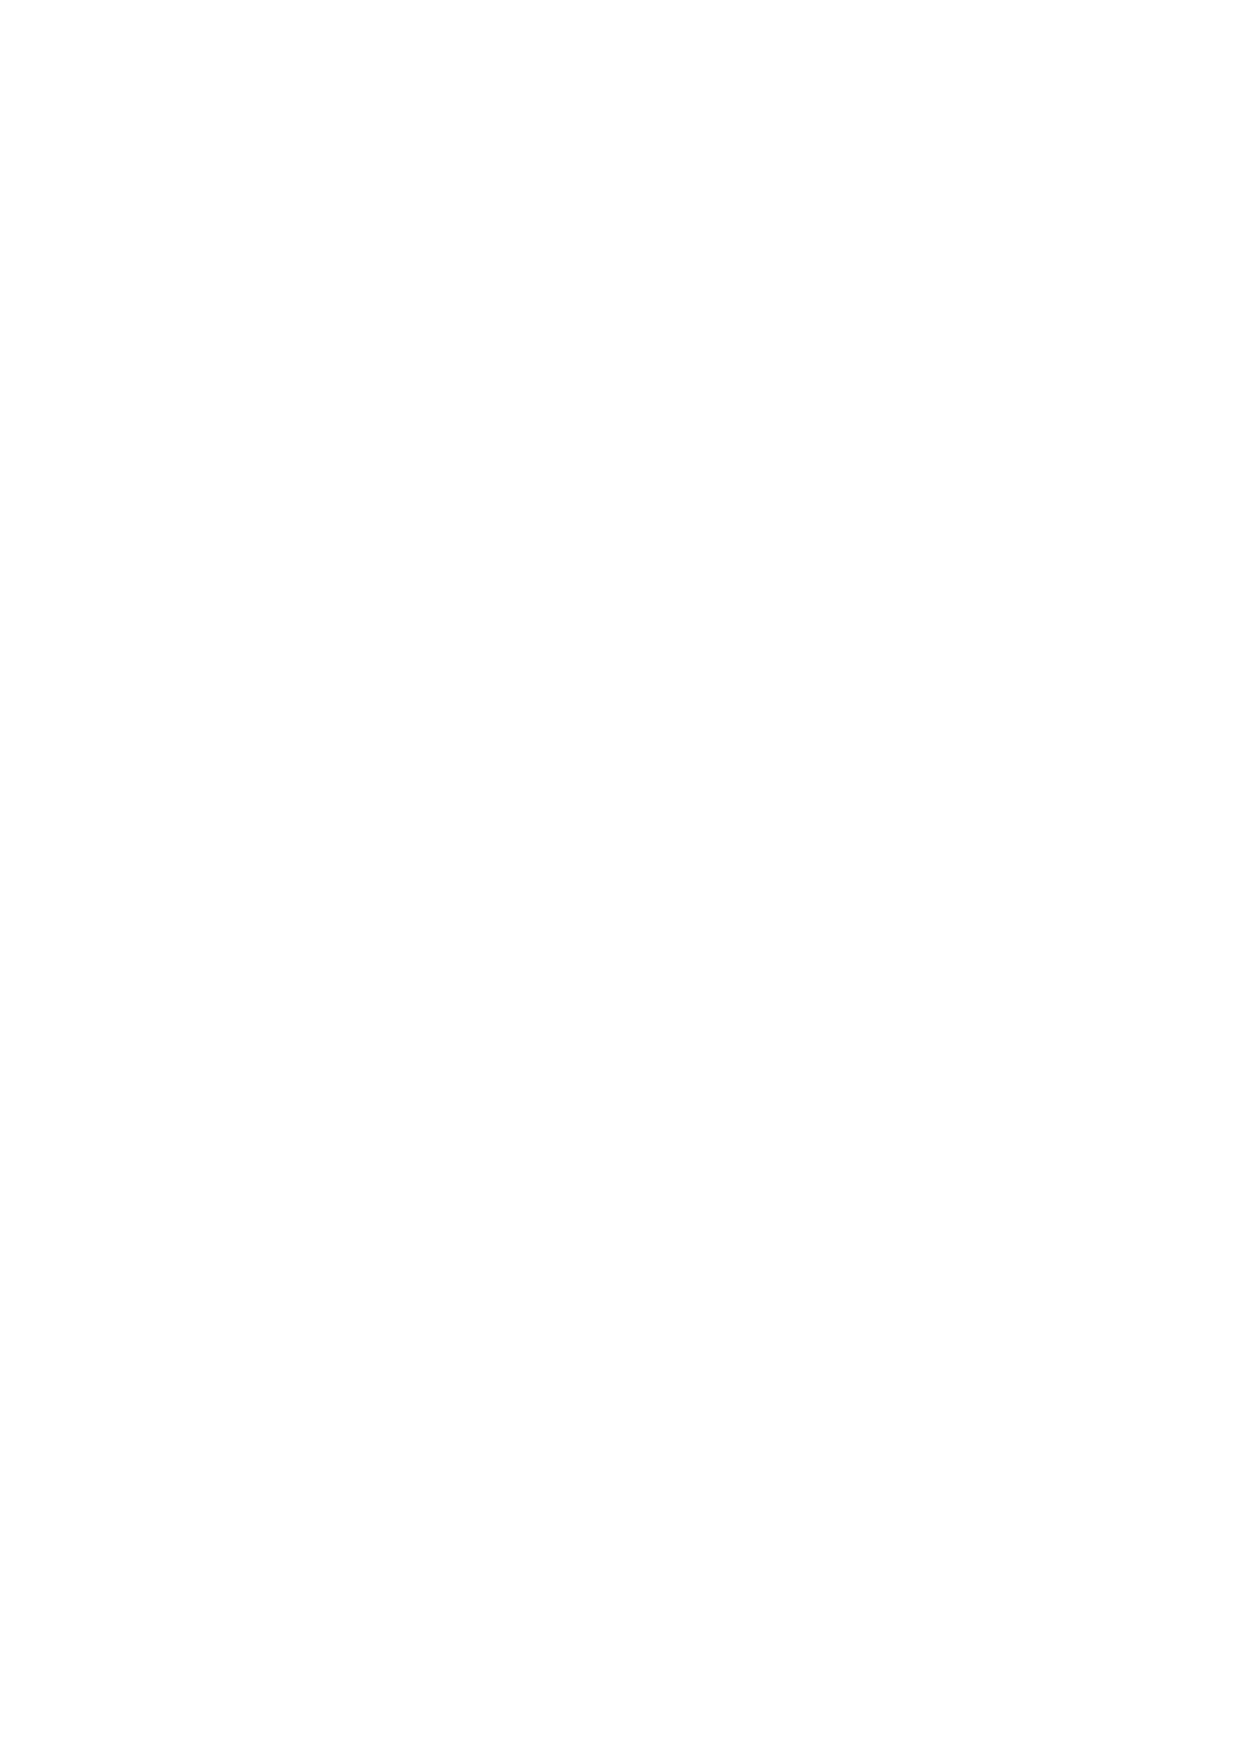
\includegraphics[scale=1.1]{\figs/postorderbt}
\end{figure}


%----------------------------------------------------------------------------------------
\section{Constructing a binary tree from a given traversal list}
\begin{itemize}
    \item In-order traversal list: $D,B,F,E,G,A,H,C,I$
        \begin{itemize}
            \item Because we know that the root is $A$ we know that everything on the right of $A$ will be the left-sub-tree and anything on the right will be the right-sub-tree.
        \end{itemize}

    \item Pre-order traversal list: $A,C,D,E,F,G,C,H,I$
        \begin{itemize}
            \item As a rule we know that the first letter will always be the root. 
            \item 
        \end{itemize}
        
    \item Post-order traversal list: $D,F,G,E,B,H,I,C,A$
        \begin{itemize}
            \item 
        \end{itemize}
\end{itemize}

% \begin{figure}[H]
    % \centering
    % 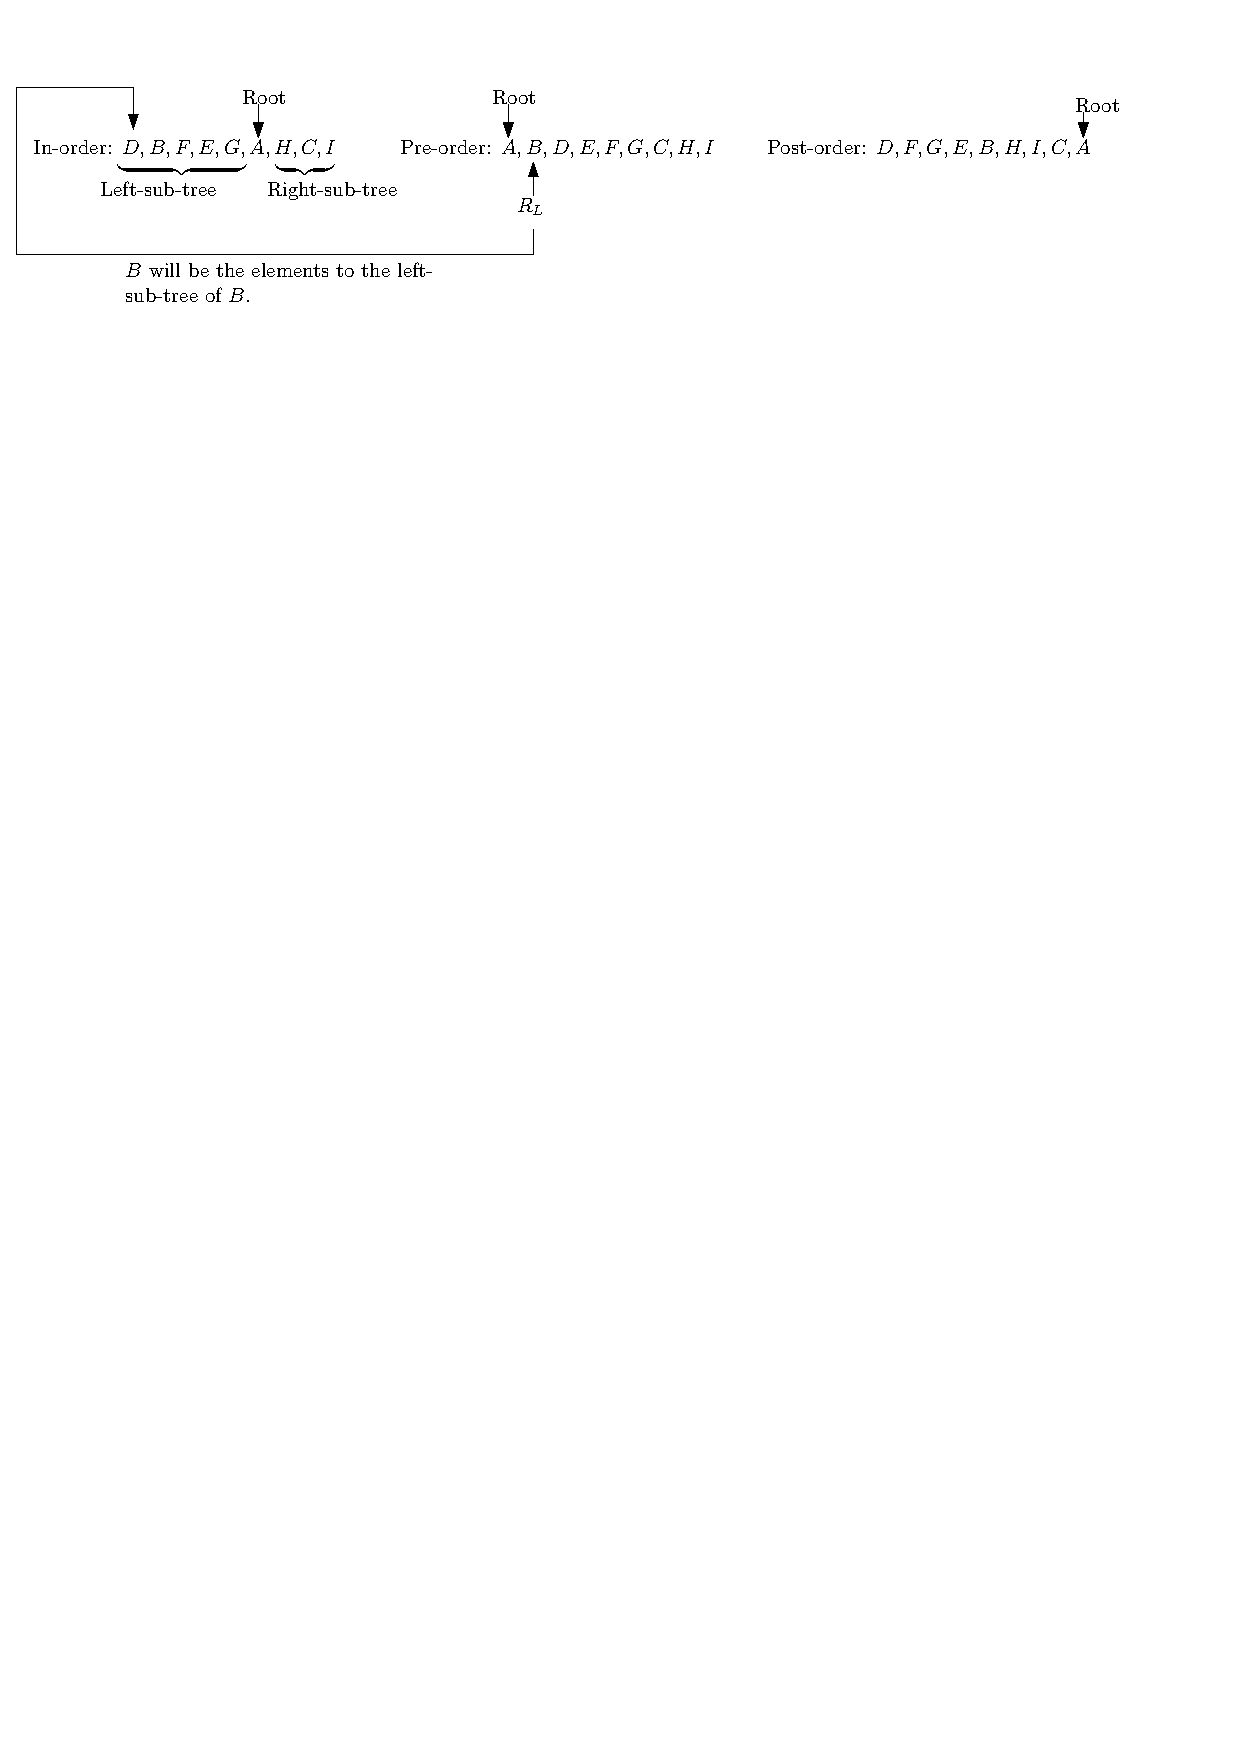
\includegraphics[]{\figs/constructionbt}
% \end{figure}
